\chapter{Uncertainty quantification in geometry reconstruction} \label{ch:uncertainty}

\vspace{-1.5 em}
\begin{addmargin}[-0.5cm]{0cm}
  \minitoc
\end{addmargin}
\hrule
\vspace{1.5 em}

In the previous two chapters, we approached the task of geometry reconstruction using two approaches, a lookup table which was only feasible for the reconstruction of triatomic molecules, and the more sophisticated optimization approach. We also ended on a rather troubling note regarding the feasibility of geometry reconstruct, namely that the reconstructed geometries exhibited unusual bond length correlations (section \ref{ssec:weirdBonds}) and that degenerate geometries can be found in large region of phase space (section \ref{sec:optimizationDegeneracies}).

In this chapter we will begin by tackling the important task of quantifying the uncertainty on our geometry reconstructions, which surprisingly has not been performed by any previous study. We will take a heuristic approach, which provides some valuble estimates on the amount of uncertainty to expect and will help resolve the issue of unusual bond length correlations. A more rigorous and sophisticated approach of uncertainty quantification in the Bayesian inference framework was attempted and although it has stagnated, the motivation and methodology of this approach will be discussed.

\section{Uncertainty on a reconstructed geometry}
The question of interest in this section is, \textit{``how does uncertainty in the measured momentum vectors affect the uncertainty of the reconstructed geometry?''} We have already calculated the uncertainty on the momentum vectors in section \ref{ssec:measurementUncertainty} but we cannot derive an analytic formula for the uncertainty on the molecular parameters or the atomic positions.

\subsection{A heuristic approach}
We will take a very basic approach here by attempting to generalize a simple result for the propagation of error through a monotonically increasing function. A monotonically increasing function is always increasing, that is, it always has a positive first derivative.

If a particular measurement $\bar{x}$ of a variable $x$ carries some uncertainty $\epsilon$ such that the true value of $\bar{x}$ lies within some interval $\bar{x} - \epsilon \le \bar{x} \le \bar{x} + \epsilon$ then the true value of some arbitrary monotonically increasing scalar function $f(x)$ that is dependent on the value of the measurement will lie within some interval
\begin{equation}
  f(\bar{x} - \epsilon) \le f(\bar{x}) \le f(\bar{x} + \epsilon)
\end{equation}

Now if we relax the condition that $f$ be a monotonically increasing function, then the true value of $f(\bar{x})$ can take on any value that $f$ attains within the interval $\bar{x} - \epsilon \le \bar{x} \le \bar{x} + \epsilon$, and we can say very generally that it lies between
\begin{equation} \label{eq:shittyInterval}
  \min_{\displaystyle \bar{x} - \epsilon \le x \le \bar{x} + \epsilon} \; f(x)
  \le f(\bar{x})
  \le \max_{\displaystyle \bar{x} - \epsilon \le x \le \bar{x} + \epsilon} \; f(x)
\end{equation}
which however, may not yield a useful interval, especially in the presence of discontinuities or divergences. However, for finite-valued and well-behaved functions that do not change rapidly within the interval $\bar{x} - \epsilon \le \bar{x} \le \bar{x} + \epsilon$, \eqref{eq:shittyInterval} may provide a useful upper bound on the uncertainty in $f(\bar{x})$. This could be particularly accurate for small neighbourhoods about $\bar{x}$. As geometry reconstruction produces physically reasonable values for the molecular parameters without any discontinuties or divergences, we will attempt to use this idea to quantify the uncertainty on a geometry's reconstruction.

Before generalizing these two ideas for multivariable measurements and functions, it will be helpful to look at this idea for the case of measurement of a vector of two variables $\bar{\mathbf{x}} = (\bar{x}_1, \bar{x}_2)$ with an uncertainty described by the vector $\bm{\epsilon} = (\epsilon_1, \epsilon_2)$ and error propagation through a vector-valued function of two variables $\mathbf{f}(\mathbf{x}) = (f_1(\mathbf{x}), f_2(\mathbf{x}))$. We will treat $\mathbf{f}(\mathbf{x})$ as non-parametric and assume that it has no analytic form, \ie~ as a \emph{black box} function as the mapping from momentum vector measurements to geometries cannot be parameterized or given in any analytical form.

In this case the true value of $\bar{\mathbf{x}}$ lies within a box described by $\bar{x}_1 - \epsilon_1 \le \bar{x}_1 \le \bar{x}_1 + \epsilon_1$ and $\bar{x}_2 - \epsilon_2 \le \bar{x}_2 \le \bar{x}_2 + \epsilon_2$ in the $x_1x_2$ plane. If both $f_1(\mathbf{x})$ and $f_2(\mathbf{x})$ depend monotonically on $x_1$ and $x_2$ then determining the range of possible values of $\mathbf{f}(\bar{x})$ would be simple. Evaluating $\mathbf{f}(\mathbf{x})$ for 
\begin{equation} \label{eq:endpoints}
\mathbf{x} \in \mathbf{x}_\mathrm{ep}
  % = \lbrace (\bar{x}_1 \pm \epsilon_1, \bar{x}_2 \pm \epsilon_2) \rbrace
  = \left\lbrace
    \begin{pmatrix} x_1 - \epsilon_1 \\ x_2 - \epsilon_2 \end{pmatrix},
    \begin{pmatrix} x_1 - \epsilon_1 \\ x_2 + \epsilon_2 \end{pmatrix},
    \begin{pmatrix} x_1 + \epsilon_1 \\ x_2 - \epsilon_2 \end{pmatrix},
    \begin{pmatrix} x_1 + \epsilon_1 \\ x_2 + \epsilon_2 \end{pmatrix}
  \right\rbrace
\end{equation}
where $\mathrm{ep}$ is an abbreviation for ``endpoints'' (as $\mathbf{x}_\mathrm{ep}$ denotes the set of endpoints for the box containing feasible values of $\mathbf{x}$ in the $x_1x_2$ plane) would produce $4$ point in the $f_1f_2$ plane, whose set we denote by $\mathbf{f}_\mathrm{ep}$ and whose rectangular boundary encloses the possible values of $f(\bar{x})$. Thus the propagation of uncertainty in this case can be thought of a mapping from a rectangle in the $x_1x_2$ plane to a rectangle in the $f_1f_2$ plane.

If $f_1$ and $f_2$ do not depend monotonically on $x_1$ and $x_2$, then values of $x_1$, $x_2$ between the endpoints may produce values of $f_1$,$f_2$ that lie outside the rectangular boundary. A further heuristic would be to not only look at the endpoints, but also a set of uniformally distributed points in the $x_1x_2$ plane within the box of possible values for $\mathbf{x}$. In this case, the propagation of uncertainty can be thought of as a mapping from a rectangle in the $x_1x_2$ plane to an arbitrary region in the $f_1f_2$ plane whose boundary may not be rectangular anymore, or even a single region. In the case of a more complicated boundary, we will generalize \eqref{eq:shittyInterval} by describing the boundary using a \emph{convex hull}. The convex hull $C$ of a set of points $S = \lbrace p_1, p_2, \dots, p_n \rbrace$ where $p_i \in \mathbb{R}^m$ for all $i$ can be expressd mathematically as
\begin{equation}
C = \left\lbrace\left.
  \sum_{i=1}^n \lambda_i p_i \right|
  \lambda_i \ge 0
  \;\; \mathrm{and} \;\;
  \sum_{i=1}^n \lambda_i = 1
  \right\rbrace
\end{equation}
An analogy in two dimensions would be to stretch a rubber band around the set of points and let it rest, its final shape being the convex hull.

%by the set of convex combinations of the points in $\mathbf{f}_\mathrm{ep}$,
%\begin{equation}
%  \displaystyle
%  \left\lbrace\left.
%  \sum_{\mathbf{f} \in \mathbf{f_i}_\mathrm{ep}}^{|\mathbf{f}_\mathrm{ep}|}
%  \alpha_i\mathbf{f_i}
%  \right| \alpha_i \ge 0 \; \mathrm{and} \;
%  \sum_i^{|\mathbf{f}_\mathrm{ep}|} \alpha_i = 1
%  \right\rbrace
%\end{equation}
%which is the convex hull of the set of points contained in $\mathbf{f}_\mathrm{ep}$, discussed further in the next subsection.

Extending this idea to our problem of geometry reconstruction, we have $9$ measurements $\bar{\mathbf{p}} = (\bar{p}_1, \dots, \bar{p}_9)$ with uncertainty $\bm{\epsilon} = (\epsilon_1, \dots, \epsilon_9)$ and we are interested in the range of possible geometries as produced by $\mathbf{g}(\mathbf{p}) = (r_{12}(\mathbf{p}), r_{23}(\mathbf{p}), \theta(\mathbf{p}))$. The possible values of the momentum components are contained within a $9$-dimensional hyperrectangle or box in momentum space, and we would like to obtain a $3$-dimensional region in phase space describing the set of possible geometries that the measurement could correspond to. Generating a set of $N$ uniformally distributed points within the $9$-dimensional box would produce $N^9$ sets of momentum vectors, each of which must be reconstructed. This represents a rather unfeasible number of reconstructions to perform, thus we will start by looking at the set of endpoints only, which contains $512$ ($2^9$) sets of momentum vectors. Attempting to reconstruct a geometry for each set of momentum vectors will ideally provide us with $512$ geometries that together give us some idea into the range of possible geometries the measurement could possibly belong to. By only reconstructing the endpoints of our box in momentum space, we may be underestimating the range of possible geometries as points within the box may produce more extreme geometries when reconstructed.

% % r_CO=131.677 pm, r_CS=187.161 pm, theta=169.42 deg
To carry out this idea for geometry reconstruction, we randomly chose a representative geometry, $(r_\mathrm{CO}, r_\mathrm{CS}, \theta) = (\SI{130}{\pico\m}, \SI{190}{\pico\m}, \SI{169}{\degree})$ that does not lie in any of the degenerate regions discussed in figure \ref{fig:OCS222DegeneracyMaps} to avoid having to account for degenerate geometries. Simulating a Coulomb explosion using this geometry as the intial condition yields a set of momentum vectors, upon which we artifically placed an uncertainty of $5\%$ for each momentum component such that $\bm{\epsilon} = 0.05\mathbf{p}$, producing $512$ sets of momentum vectors corresponding to the corners of the $9$-dimensional box in momentum space, that is, a 9-dimensional version of \eqref{eq:endpoints}. Reconstructing a geometry for each set of momentum vectors, we obtain $512$ geometries and all $512$ sets of momentum vectors were successfully mapped to a unique geometry. Histograms showcasing the bond length and bond angle distributions of these reconstructed geometries are plotted in figure \ref{fig:OCS222Uncertainty} along with scatter plots showcasing the bivariate relationships between the three molecular parameters.

\begin{figure}
  \centering
  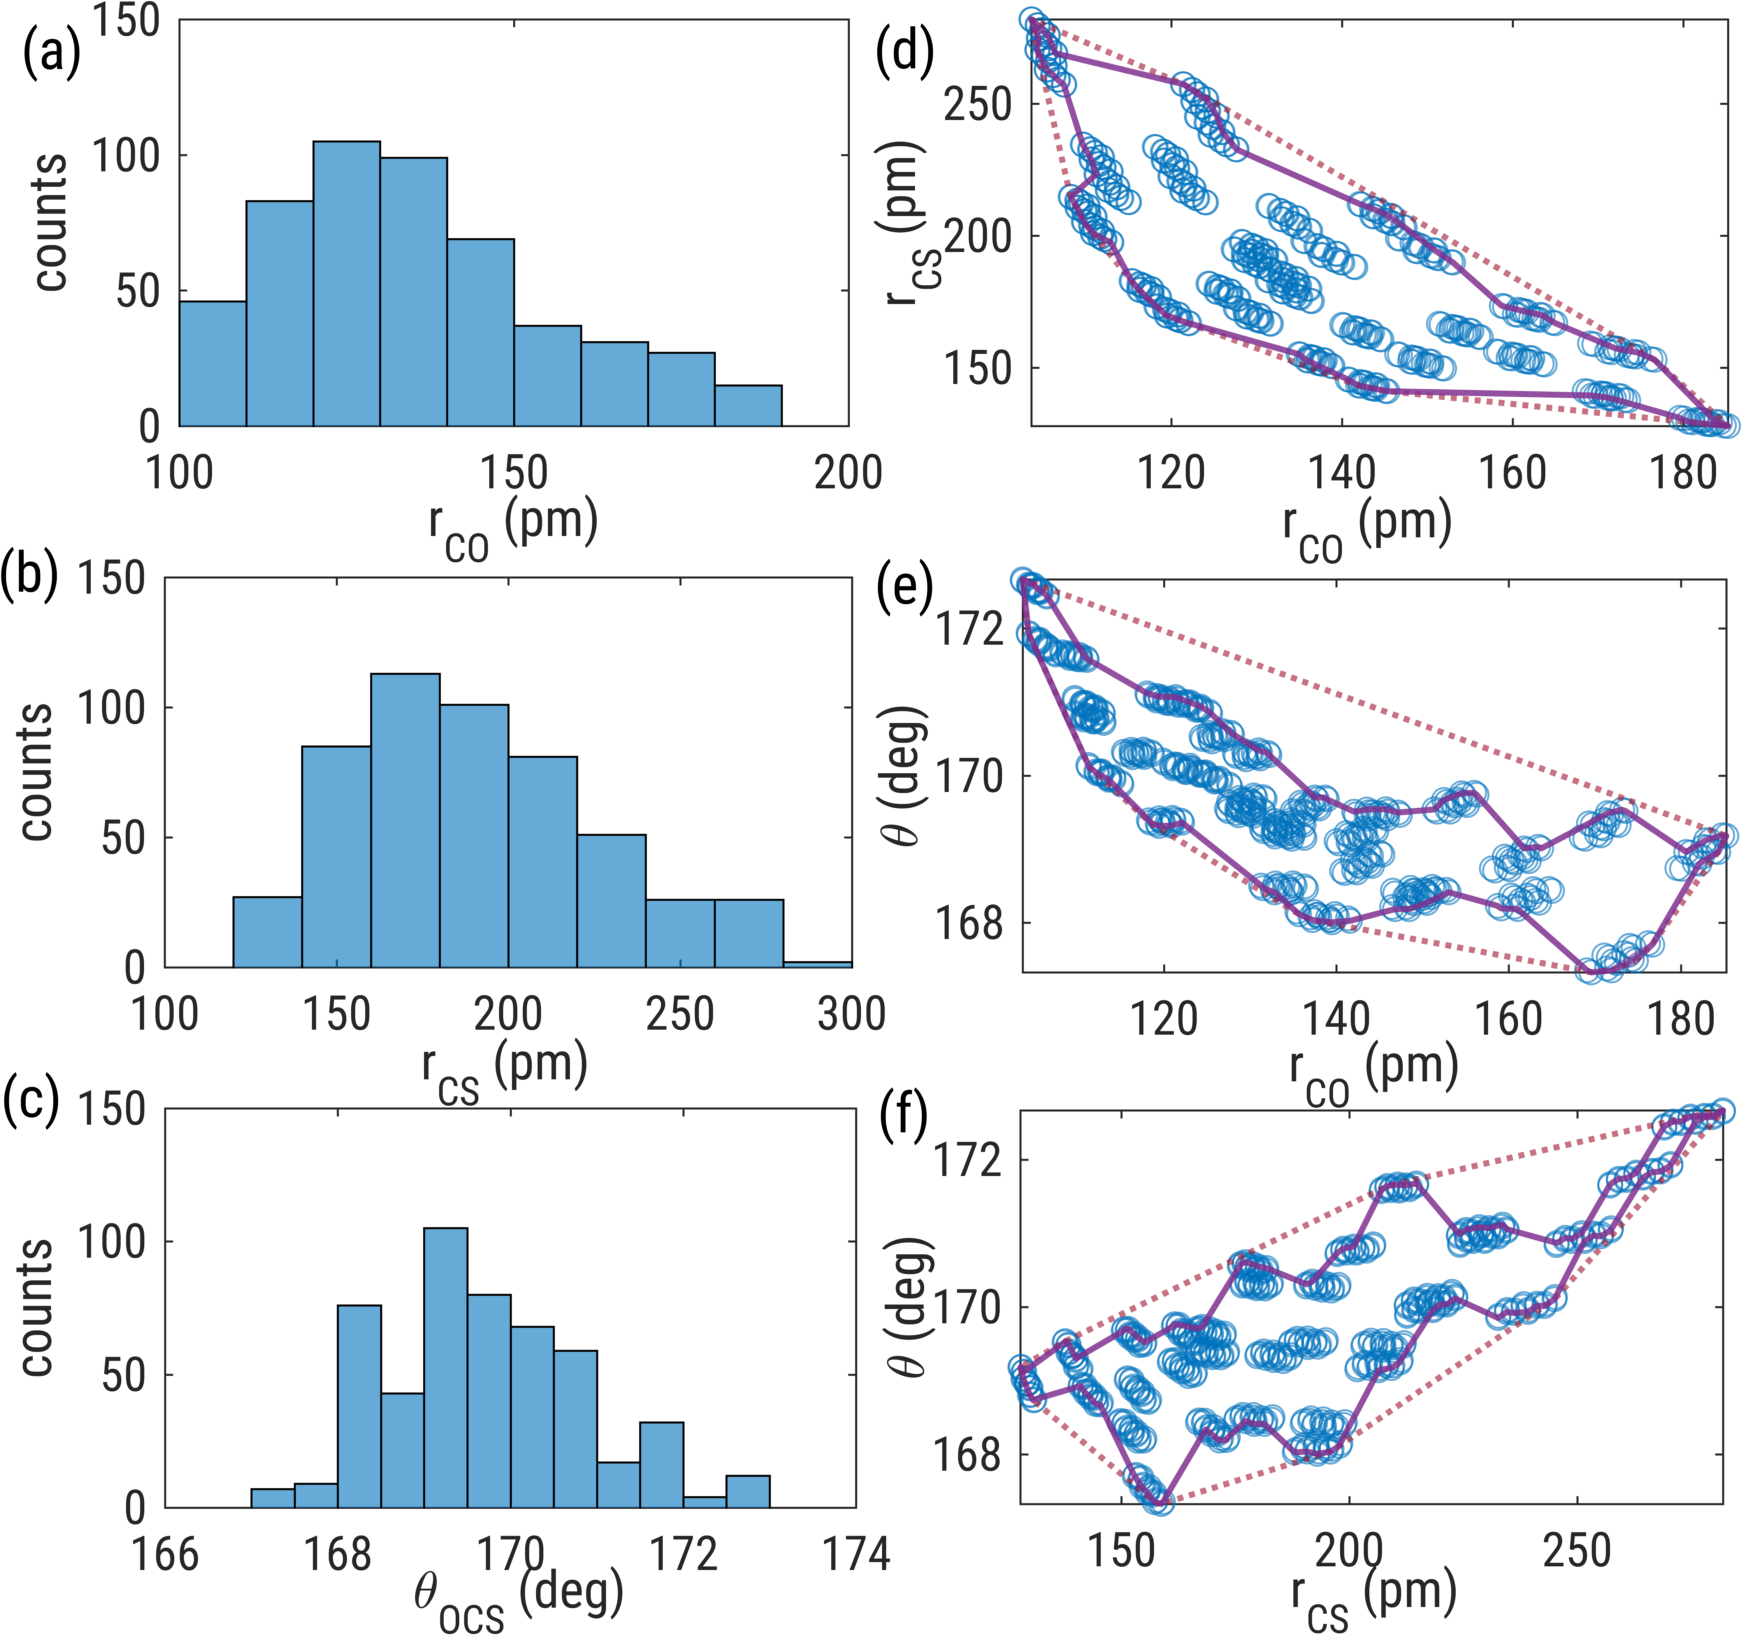
\includegraphics[width=\textwidth]{Plots/OCS222Exploration1_5percent}
  \caption[A heuristic estimate on the range of possible \ch{OCS} $(2,2,2)$ geometries that may be reconstructed assuming a true geometry of $(r_\mathrm{CO}, r_\mathrm{CS}, \theta) = (\SI{130}{\pico\m}, \SI{190}{\pico\m}, \SI{169}{\degree})$ and $5\%$ uncertainty on the measured momentum vectors.]
  {A heuristic estimate on the range of possible \ch{OCS} $(2,2,2)$ geometries that may be reconstructed assuming a true geometry of $(r_\mathrm{CO}, r_\mathrm{CS}, \theta) = (\SI{130}{\pico\m}, \SI{190}{\pico\m}, \SI{169}{\degree})$ and $5\%$ uncertainty on the measured momentum vectors. Histograms showcase the (a) \ch{C-O} bond length, (b) \ch{C-S} bond length, and (c) bond angle distributions of the reconstructed geometries. Scatter plots showcase the bivariate relationships between (d) $r_\mathrm{CO}$ and $r_\mathrm{CS}$, (e) between $r_\mathrm{CO}$ and $\theta$, and (f) between $r_\mathrm{CS}$ and $\theta$. Each reconstructed geometry is plotted as an open blue circle. The boundary of the set of reconstructed geometries is calculated using two methods and plotted; The dotted red line denotes the convex hull and the solid purple line denotes the alpha shape (using (d) $\alpha=15$, (e) $\alpha=22$, and (f) $\alpha=30$) of the set of points.}
  \label{fig:OCS222Uncertainty}
\end{figure}

We immediately see that a strikingly wide range of geometries are reconstructed assuming the momentum components carry an uncertainty of only $5\%$. Inspection suggests that the bond length and bond angle distributions roughly form a Gaussian distribution about the true parameters. The distributions encompass a wide range of possible bond lengths, \SI{80}{\pico\m} for the \ch{C-O} bond and \SI{175}{\pico\m} for the \ch{C-S} bond. The variability in the bond angle is not as extreme, encompassing a \SI{6}{\degree} range of possible bond angles.

The bivariate relationships shown in figures \ref{fig:OCS222Uncertainty}(d)-(f) suggest the range of possible geometries. Interestingly, the bond length correlation in figure \ref{fig:OCS222Uncertainty}(d) seems to follow a reciprocal relationship, a strikingly similar one to the unusual one observed in the reconstructions of experimental data. This suggests that uncertainty in the momentum measurments may lead to the reconstruction of a geometry with asymetrically stretched bonds, and that the unusual relationship we observed in section \ref{ssec:weirdBonds} may have been a manifestation of measurement uncertainty and due to the highly sensitive nature of geometry reconstruction.

Placing a larger uncertainty on the momentum vector components further stretches the shape of the set of points in figure \ref{fig:OCS222Uncertainty}(d), modifying it to further resemble the more extreme reciprocal relationship between $r_\mathrm{CO}$ and $r_\mathrm{CS}$ found for longer pulse lengths (see figures \ref{fig:OCS22230fsMOGeometryPairs} -- \ref{fig:OCS222100fsLTGeometryPairs}). 

Exposing the molecule to longer laser pulses provides a longer amount of time for the molecule to rearrange and may impart the atomic fragments with a larger initial momentum, thus decreasing the certainty with which the measured momentum vectors correspond to the true geometry. If we take a reciprocal relationship to be a signature indicating that too much measurement uncertainty is present for trustworthy geometry reconstructions, then we must conclude that even an uncertainty as low as a few parts per hundred in the momentum vector components is ``too much'' and that geometry reconstruction using Coulomb explosion imaging is unfeasible under such conditions.

We may use the area formed by the set of points in figures \ref{fig:OCS222Uncertainty}(d)-(f), plotted as red dotted lines by the use of a convex hull, as a quantitative measure of uncertainty. Another boundary may be provided by the \emph{alpha shape} of the set of points, plotted as solid purple lines.

An interesting observation resulting from the close inspection of the open blue circles in figures \ref{fig:OCS222Uncertainty}(d)-(f) is the clustering of geometries in phase space as geometries seem to cluster in little groups. Each geometry is actually paired with one other geometry (close inspection of the open blue circles should reveal that they appear in pairs, sometimes appearing as a single blurred circle) so that $256$ points are visible unless the scatter plots are very closely inspected. As we picked one of two extreme values, $\bar{p} - \epsilon$ and $\bar{p} + \epsilon$ for each momentum component, each component may be responsible for the ``splitting of the geometries'' into pairs or clusters. This suggests that some uncertainty in certain momentum components may have a greater effect on the uncertainty of reconstructed geometries.

\subsection{Convex hulls and alpha shapes}
To quantify the uncertainty in the geometries, we will use two useful concepts from computational geometry, namely convex hulls and alpha shapes, which allow us to assign a shape and a volume to a set of points, and thus provide an additional hueristic quantitative measure of uncertainty.

The convex hull of a set of points $S$ is the set of all convex combinations of its points. An analogy would be to stretch a rubber band around the set of points and let it rest, its final shape being the convex hull.

Many algorithms exist to calculate the convex hull of a set of points, especially in 2 or 3 dimensions.

The concept of an alpha shape is a generalization of the convex hull first introduced by \citet{Edelsbrunner83} for two-dimensional shapes, then for three-dimensional shapes \citep{Edelsbrunner94}. Interestingly, alpha shapes have been used to analytically compute shapes for macromolecules such proteins and estimate their molecular areas and volume \citep{Liang98}. An interesting analogy of alpha shapes uses ice cream scoopers.

The nice thing about convex hulls is that they are unique for each set of points, while multiple distinct alpha shapes exist. This is a desirable property of alpha shapes as there is no formal concept of shape so no algorithm can determine the correct shape for a set of points. However, the concept allows for an $\alpha$ to be picked that produces the most desirable shape. 

While a very haphazard measure of uncertainty, they are much easier to employ than the sophisticated uncertainty quantification framework of Bayesian inference (section \ref{sec:uncertaintyBayesian}) and will come in handy when we perform some exploratory uncertainty analysis in section \ref{sec:uncertaintyAnalysis}. Our needs are rather basic at this point.

We end by providing a cool figure showcasing the three-dimensional convex hull and alpha shape in molecular phase space.

% figure Z here

\section{Determining the sources of uncertainty}
We saw in figure X that certain momentum components may have a much greater effect on the uncertainty on a reconstructed geometry, or that geometry reconstruction is much more sensitive to certain momentum components than others.

We will attempt to explore this effect and pinpoint the momentum components responsible for introducing the most and the least uncertainty. To do this for the oxygen's $p_x$ component for example, we will look at the $256$ sets of momentum vectors that represent the extreme end and plot their position in the $r_\mathrm{CO}-r_\mathrm{CS}$ plane in phase space. Doing this for each component, we should have $9$ plots in total.

% figure Y here

We definitely see that some components are more responsible than others. For example, the A component seems largely responsible for variability in $r_\mathrm{CO}$ and the B component seems responsible for variability in the $r_\mathrm{CS}$ component. Interestingly, removing the C component seems to produce a plot almost exactly like the one in figure X, suggesting that uncertainty in C introduces a negligible amount of uncertainty in the reconstructed geometries.

This result has implications for the design and operation of Coulomb explosion imaging experiments, especially if the determination of molecular structure is a concern. The CEI apparatus could be built with the aim of minimizing certain momentum components. The laser's polarization may also have an effect.

The exact dependence observed in figure Y may be due to experimental considerations. Or choice of momentum convention? Further investigation is certainly warranted.

\section{Exploratory uncertainty analysis} \label{sec:uncertaintyAnalysis}
Let's put a range of uncertainties on the momentum vectors and observe how much uncertainty we have on the reconstructed geometries. We will use the widths of the distributions and the convex hull and alpha shape areas and volumes to quantify the uncertainty with the aim of finding how uncertainty in geometry reconstruction varies as a function of uncertainty in the momentum vectors.

% Various figures here

Interestingly, we are always able to reconstruct the geometry.

\section{Uncertainty quantification using Bayesian inference} \label{sec:uncertaintyBayesian}
The heuristic uncertainty quantification performed in the previous three sections has provided some significant insights on the problem of geometry reconstruction, and emphasized the large effect that measurement uncertainty must have played in our reconstruction of experimental data. This emphasizes the importance of tackling the task of uncertainty quantification in a rigorous and sophisticated manner, in which case the Bayesian inference framework provides the answer.

% Philosophy? objective vs. subjective Bayes, frequentist vs. Bayesian, etc.
The Bayesian point of view provides a more natural and intuitive way of thinking about uncertainty in the physical sciences.

% Why Bayesian inference is perfect for inverse problems.

Bayesian statistics actually predates the much more commonly taught frequentist statistical methods but has made a strong resurgence in recent years due to rising computational abilities and more recently, available software for parameter estimation in statistical models using Markov chain Monte Carlo.

\subsection{Elementary concepts}
% Ideas?: credibility, models, parameters, distributions.
% Theory?: Bayes Theorem, prior predictive, posterior, posterior mode (read up).
% Bayes’ theorem: we just need to do a multi-dimensional integral

\subsection{Markov chain Monte Carlo}
% The basic idea
Performing the multi-dimensional integral can be very difficult. The integral is usually approximated using Markov Chain Monte Carlo.
% Markov Chain Monte Carlo: transition kernel, checking for convergence, Metropolis-Hastings algorithm, Gibbs Sampling, Hamiltonian MCMC

\subsection{Other Bayesian methods}
Uncertainty quantification for inverse problems in the Bayesian framework.

% Tikhonov regularization? Actually Bayesian inversion is a great alternative?

% MMMGRUBS alternative idea: Time evolve the system backwards from the measurement using a Kalman filter to keep track of the error in the geometry. My guess: The magnitude of the error will be much larger than the physical size of the molecule.

\section{Conclusions}